%%%%%%%%%%%%%%%%%%%%%%%%%%%%%%%%%%%%%%%%%%%%%%%%%%%%%%%%%%%%%%%%%%%%%%%%%%%%%%%%
% Univerzita Komenskeho - Thesis template
% Based on "Vnutorny predpis c. 12/2013"
%%%%%%%%%%%%%%%%%%%%%%%%%%%%%%%%%%%%%%%%%%%%%%%%%%%%%%%%%%%%%%%%%%%%%%%%%%%%%%%%

%%%%%%%%%%%%%%%%%%%%%%%%%%%%%%%%%%%%%%%%%%%%%%%%%%%%%%%%%%%%%%%%%%%%%%%%%%%%%%%%
% Global document settings
%%%%%%%%%%%%%%%%%%%%%%%%%%%%%%%%%%%%%%%%%%%%%%%%%%%%%%%%%%%%%%%%%%%%%%%%%%%%%%%%
% Cl.7/2 - font size 12pt, portrait, A4
% Cl.7/6 - single side printing
\documentclass[a4paper,12pt,oneside,final]{memoir}
% Cl.7/2 - 1.5x line spacing
\OnehalfSpacing

%%%%%%%%%%%%%%%%%%%%%%%%%%%%%%%%%%%%%%%%%%%%%%%%%%%%%%%%%%%%%%%%%%%%%%%%%%%%%%%%
% Page geometry
%%%%%%%%%%%%%%%%%%%%%%%%%%%%%%%%%%%%%%%%%%%%%%%%%%%%%%%%%%%%%%%%%%%%%%%%%%%%%%%%
%\setstocksize{297mm}{210mm}
%\settrimmedsize{297mm}{210mm}{*}
\settypeblocksize{247mm}{155mm}{*}
% Cl.7/3 - 3.5cm left, 2cm right
% Cl.7/3 - 2.5cm top, 2.5cm bottom
\setlrmarginsandblock{3.5cm}{2cm}{*}
\setulmarginsandblock{2.5cm}{2.5cm}{*}
\checkandfixthelayout

%%%%%%%%%%%%%%%%%%%%%%%%%%%%%%%%%%%%%%%%%%%%%%%%%%%%%%%%%%%%%%%%%%%%%%%%%%%%%%%%
% Language, encoding, fonts
%%%%%%%%%%%%%%%%%%%%%%%%%%%%%%%%%%%%%%%%%%%%%%%%%%%%%%%%%%%%%%%%%%%%%%%%%%%%%%%%
% TODO pick fonts
%\usepackage{charter}


\usepackage{fontspec}
\usepackage{polyglossia}
\setdefaultlanguage{english}
\usepackage{csquotes}
%%%%%%%%%%%%%%%%%%%%%%%%%%%%%%%%%%%%%%%%%%%%%%%%%%%%%%%%%%%%%%%%%%%%%%%%%%%%%%%%
% Important packages
%%%%%%%%%%%%%%%%%%%%%%%%%%%%%%%%%%%%%%%%%%%%%%%%%%%%%%%%%%%%%%%%%%%%%%%%%%%%%%%%
\usepackage{microtype} % Typographical improvements
\usepackage{booktabs} % Better looking tables
\usepackage{pdfpages} % Include PDFs
\usepackage[bottom]{footmisc} % Move footnotes to the bottom

\usepackage[binary-units=true]{siunitx} % SI units + binary prefix (Mi, Gi, ...)
\usepackage{xspace} % Smart space for macros

% Figures
\newsubfloat{figure} % Allow subfigures
\usepackage{graphicx} % Images
\usepackage{threeparttable} % Tables
\usepackage{rotating} % Sideways figures

% TikZ illustrations
\usepackage{tikz}
%\usepackage{tikz-qtree}
%\input{tikz-settings}

% Math related
\usepackage{amsmath,amsthm}
\usepackage{amsfonts}
\usepackage{mathtools}
\usepackage{bm, mathrsfs}

% Custom symbols imported from fonts
%\input{symbols}

% TODO? remove amsfonts, use unicode-math
% TODO? but change the ugly fonts
%\usepackage[]{unicode-math}

% Algoritms / pseudo-code
\usepackage[chapter]{algorithm}
\makeatletter \renewcommand{\ALG@name}{Algoritmus}
\usepackage[noend]{algpseudocode} % No explicit "end function" line
\newcommand*\AlgLet[2]{\State #1 $\gets$ #2} % X <- Y assignment 

% Code syntax highlighting
\usepackage[chapter]{minted}
\usemintedstyle{tango}
%\renewcommand\listingscaption{Zdrojový kód}

\usepackage{multirow}
\usepackage{arydshln}

\usepackage{float}

%%%%%%%%%%%%%%%%%%%%%%%%%%%%%%%%%%%%%%%%%%%%%%%%%%%%%%%%%%%%%%%%%%%%%%%%%%%%%%%%
% Bibliography
%%%%%%%%%%%%%%%%%%%%%%%%%%%%%%%%%%%%%%%%%%%%%%%%%%%%%%%%%%%%%%%%%%%%%%%%%%%%%%%%
\usepackage[backend=bibtex, natbib=true]{biblatex}
\addbibresource{research.bib}

% Style tweaks
\renewcommand*{\finalnamedelim}{\addcomma\addspace}
\renewcommand*{\labelnamepunct}{\addcolon\addspace}
\renewcommand*{\newunitpunct}{\addcomma\addspace}
\DeclareFieldFormat[article,inbook,incollection,inproceedings,patent,thesis,unpublished]{title}{\textit{#1}}
% Add all bibliography uncited in text
\nocite{*}

%%%%%%%%%%%%%%%%%%%%%%%%%%%%%%%%%%%%%%%%%%%%%%%%%%%%%%%%%%%%%%%%%%%%%%%%%%%%%%%%
% Misc packages
%%%%%%%%%%%%%%%%%%%%%%%%%%%%%%%%%%%%%%%%%%%%%%%%%%%%%%%%%%%%%%%%%%%%%%%%%%%%%%%%
\usepackage{lipsum} % Lorem ipsum (for testing)

%\usepackage[color=white]{todonotes} % print mode
\usepackage{todonotes}

% XeLaTeX and BibTex
\usepackage{metalogo}
%\usepackage{dtklogos}

\usepackage{ccicons}

%%%%%%%%%%%%%%%%%%%%%%%%%%%%%%%%%%%%%%%%%%%%%%%%%%%%%%%%%%%%%%%%%%%%%%%%%%%%%%%%
% Setup document preferences
%%%%%%%%%%%%%%%%%%%%%%%%%%%%%%%%%%%%%%%%%%%%%%%%%%%%%%%%%%%%%%%%%%%%%%%%%%%%%%%%
% Chapter style
\makeatletter

\newlength{\numberheight}
\setlength{\numberheight}{\beforechapskip}

\newlength{\barlength}
\newlength{\chnumwidth}

\newlength{\namenumsep}
\setlength{\namenumsep}{0.5em}

\newlength{\numbarsep}
%\setlength{\numbarsep}{1em}
\setlength{\numbarsep}{10em}

% Modified from 'veelo' style in memoir and
% https://tex.stackexchange.com/questions/69656/right-align-chapter-number-to-the-chapter-name-when-using-memoir-with-veelo-styl

\makechapterstyle{myveelo}{%
    \setlength{\afterchapskip}{40pt}
    \renewcommand*{\chapterheadstart}{\vspace*{40pt}}
    \renewcommand*{\afterchapternum}{\par\nobreak\vskip 25pt}
    \renewcommand*{\chapnamefont}{\normalfont\LARGE\flushright}
    \renewcommand*{\chapnumfont}{\normalfont\HUGE}
    \renewcommand*{\chaptitlefont}{\normalfont\HUGE\bfseries\flushright}
    \renewcommand*{\chapternamenum}{}
    
    \setlength{\midchapskip}{\paperwidth}
    \addtolength{\midchapskip}{-\textwidth}
    \addtolength{\midchapskip}{-\spinemargin}
    
    \setlength{\barlength}{\midchapskip}
    \addtolength{\barlength}{-\numbarsep}
        
    \renewcommand*{\printchaptername}{%
        \settowidth{\chnumwidth}{\resizebox{!}{\numberheight}{\chapnumfont \thechapter}}%
        \chapnamefont\MakeUppercase{\@chapapp}%
        \hspace*{\chnumwidth}%
        \hspace*{\namenumsep}%
    }
    
    \renewcommand*{\printchapternum}{%
        \makebox[0pt][l]{
            \settowidth{\chnumwidth}{\resizebox{!}{\numberheight}{\chapnumfont \thechapter}}%
            \hspace*{-\chnumwidth}%
            \resizebox{!}{\numberheight}{\chapnumfont \thechapter}%
            \hspace*{\numbarsep}%
            \rule{\barlength}{\numberheight}%
    }}%
}

\makeatother
\chapterstyle{myveelo} % TODO pick - veelo, madsen, ?

% Subsections and higher - numbered and in TOC
\setsecnumdepth{subsection}
\maxtocdepth{subsection}

% Headers / footers
\pagestyle{ruled}
% https://tex.stackexchange.com/questions/176472/identical-marks-in-header-with-onesided-memoir/176484?noredirect=1#176484
% https://tex.stackexchange.com/questions/59565/on-testing-two-fully-expanded-character-strings-for-equality
\usepackage{pdftexcmds} 
\makeatletter
\newcommand*{\test}[2]{%
  \ifnum\pdf@strcmp{#1}{#2}=\z@ \relax \else #2 \fi
}
\makeatother
\makeoddhead{ruled}{\sffamily\leftmark}{}{\sffamily\test{\leftmark}{\rightmark}}

% Create custom plain page style with pagenumbers on right instead of centered
\makepagestyle{plainright}
\makeoddfoot{plainright}{}{}{\thepage}
\aliaspagestyle{chapter}{plainright}

% Custom caption rules
\newfixedcaption{\figcaption}{figure}
\newfixedcaption{\algcaption}{algorithm}

% Custom theorem enviroments
\newtheorem{theorem}{Theorem}[section]
\newtheorem{lema}[theorem]{Lema}

\setlength{\epigraphwidth}{6cm}

%%%%%%%%%%%%%%%%%%%%%%%%%%%%%%%%%%%%%%%%%%%%%%%%%%%%%%%%%%%%%%%%%%%%%%%%%%%%%%%%
% Macros
%%%%%%%%%%%%%%%%%%%%%%%%%%%%%%%%%%%%%%%%%%%%%%%%%%%%%%%%%%%%%%%%%%%%%%%%%%%%%%%%
\newcommand{\unnumberedchapter}[1]{
    \chapter*[#1]{#1}
    \addcontentsline{toc}{chapter}{#1}
}

% Generic shortcuts
\newcommand{\bigO}[1]{\ensuremath{\mathcal{O}(#1)}}
\newcommand{\inlcode}[1]{\texttt{#1}\xspace}

% Shortcuts specific to this document
\newcommand{\etal}{et al.\@\xspace}
% https://tex.stackexchange.com/questions/42619/x-mark-to-match-checkmark/42620#42620
%\usepackage{pifont}% http://ctan.org/pkg/pifont
%\newcommand{\cmark}{\ding{51}}%
%\newcommand{\xmark}{\ding{55}}%	
\newcommand{\cmark}{On}%
\newcommand{\xmark}{Off}%


%%%%%%%%%%%%%%%%%%%%%%%%%%%%%%%%%%%%%%%%%%%%%%%%%%%%%%%%%%%%%%%%%%%%%%%%%%%%%%%%
% Include document settings (title, name, ...)
%%%%%%%%%%%%%%%%%%%%%%%%%%%%%%%%%%%%%%%%%%%%%%%%%%%%%%%%%%%%%%%%%%%%%%%%%%%%%%%%
\def \settingsSchool{Univerzita Komenského v Bratislave}
\def \settingsFaculty{Fakulta matematiky, fyziky a informatiky}

\def \settingsTitle{Use of SAT Solvers in Cryptanalysis}
\def \settingsAuthor{Bc. Ladislav Pápay}
\def \settingsYear{2016}

\def \settingsProgramme{TODO Informatika}
\def \settingsField{TODO KOD 2508 Informatika}
\def \settingsDepartment{Katedra Informatiky FMFI}
\def \settingsAdvisor{doc. RNDr. Martin Stanek, PhD.}

\def \settingsAISfile{ais-zadanie-export.pdf}

%%%%%%%%%%%%%%%%%%%%%%%%%%%%%%%%%%%%%%%%%%%%%%%%%%%%%%%%%%%%%%%%%%%%%%%%%%%%%%%%
% Hyperref setup
%%%%%%%%%%%%%%%%%%%%%%%%%%%%%%%%%%%%%%%%%%%%%%%%%%%%%%%%%%%%%%%%%%%%%%%%%%%%%%%%
\usepackage[hidelinks]{hyperref}
\hypersetup{
    unicode=true,
    pdftitle={\settingsTitle},
    pdfauthor={\settingsAuthor},
    bookmarksnumbered=true,     
    bookmarksopen=true,         
    bookmarksopenlevel=1,       
    pdfpagemode=UseOutlines
}

%%%%%%%%%%%%%%%%%%%%%%%%%%%%%%%%%%%%%%%%%%%%%%%%%%%%%%%%%%%%%%%%%%%%%%%%%%%%%%%%
% Start of document
%%%%%%%%%%%%%%%%%%%%%%%%%%%%%%%%%%%%%%%%%%%%%%%%%%%%%%%%%%%%%%%%%%%%%%%%%%%%%%%%
\begin{document}
\frontmatter
    %\newcommand{\coverTop}{
    \begin{center}
        {\textbf \Large \textsc {\settingsSchool \\ \settingsFaculty}}
        \vfill
        {\LARGE \em \settingsTitle}
        \\
        \medskip
        {\large \textsc{Master's Thesis}}
    \end{center}
}

\newcommand{\coverCenter}{
    \begin{tabular}{l l}
        \textbf{Study programme:} & \settingsProgramme \\
        \textbf{Study field:} & \settingsField \\
        \textbf{Department:} & \settingsDepartment \\
        \textbf{Supervisor:} &  \settingsAdvisor
    \end{tabular}
}

\newcommand{\coverBottom}{
    \begin{center}
        {\settingsYear \hfill \settingsAuthor}
    \end{center}
}

\thispagestyle{empty}
\coverTop
\vfill
\begin{center}
    {\settingsYear \hfill \settingsAuthor}
\end{center}
\newpage

\thispagestyle{empty}
\coverTop
\vfill
\coverCenter
\vfill
\begin{center}
    {Bratislava, \settingsYear \hfill \settingsAuthor}
\end{center}
\newpage



    %\includepdf[pages=1]{\settingsAISfile}
    %\newpage
    
    %\thispagestyle{plainright}
    %\input{thanks}
    %\newpage
    %\thispagestyle{plainright}
    %\input{disclaimer}
    %\newpage
    
    
    %\input{abstracts}
    %\newpage
    
    %\tableofcontents*
    %\newpage
    %\listoffigures*
    
\mainmatter
    %\begin{abstract}
\unnumberedchapter{Abstract}
SAT solvers are a universal tool for finding solutions to boolean satisfiability problems.
In the past they have also been used for cryptographic problems, such as finding preimages for hash functions or obtaining the key for stream ciphers.
However these solutions are not easily reusable or modifiable.

In our work we create a modeling library that allows simple creation of SAT instances.
We specifically focus on various problems related to cryptographic hash functions, however the library is generic enough that it can be used for other purposes as well.

Using this library we create models for several cryptographic hash functions.
Various SAT solvers, optimizations and heuristics are evaluated on these models to compare their performance.
These include the use of the \emph{Espresso} logic minimizer to reduce the instance size, forcing custom variable branching order with help of modified SAT solvers and others.

%\keywords{SAT, cryptography, hash functions, heuristics}
%TODO keywords
%\end{abstract}
\unnumberedchapter{Abstrakt}
SAT solvery sú univerzálny nástroj pre hľadanie riešení boolovských problémov spl\-ni\-teľ\-no\-sti.
V minulosti boli používané aj na kryptografické problémy, ako napríklad hľadanie vzoru hašovacích funkcií alebo kľúča prúdových šifier.
Avšak tieto prístupy a riešenia nie je možné ľahko upraviť a opätovne využiť.

V našej práci sme vytvorili knižnicu pre jednoduché modelovanie SAT inštancií.
Sústredili sme sa špeciálne na rôzne problémy súvisiace s kryptografickými hašovacími funkciami, ale vytvorená knižnica je dostatočne všeobecná a je ju možné použiť aj na iné účely.

S pomocou tejto knižnice sme vytvorili modely pre niekoľko kryptografických hašovacích funkcií.
Ďalej sme testovali niekoľko SAT solverov, optimalizácií a heuristík a porovnávali sme ich efektivitu.
Okrem iného sme využívali logický minimalizér \emph{Espresso} na redukciu veľkosti inštancií, a tiež vlastné poradie vetvenia pri ohodnocovaní premenných s pomocou upraveného SAT solveru.
\chapter{Introduction}
\section{SAT solvers}
\emph{SAT solvers} (shortened from \emph{satisfiability}) are programs which take a boolean satisfiability problem and a find solution or solutions to this problem.
The problem, which we will call an \emph{instance}, consists of a number of variables and boolean clauses composed of these variables.
The solution, if it exists, is an assignment of truth values to the variables such that the clauses are satisfied.
If no such assignment exists the instance is called \emph{unsatisfiable}.

Most modern SAT solvers expect input in \emph{conjunctive normal form} in which all clauses are disjunctions of literals (literal is either a variable or a negation of a variable, and at least one literal must be true) and the instance is a conjunction of such clauses (all clauses must be true).
As the name suggests this is a normal form, which means every boolean expression can be converted to an equivalent one that satisfies these requirements.
Thus we will from now on only consider such instances without loss of generality.

By modeling a decision problem as a SAT instance we can take advantage of the advanced optimizations and heuristics employed by modern SAT solvers.
Examples of such uses in practice include formal program verification, model checking or even routing of connections in microchips.
%TODO refs for use cases

\subsection{Implementation}
Since SAT is an $NP$-complete language and assuming $P \neq NP$ we can not in general find solutions in polynomial time.
A simple exponential time algorithm is to try every possible boolean truth assignment.
To remember which assignments have been tried and which have not we can implement this algorithm as a recursive backtracking, where for every input variable we try in turn both possible values.
This will only require linear memory to implement.

While there are no known algorithms that perform asymptotically better in he worst case, we can still improve on this simple exponential time algorithm significantly by avoiding paths that are guaranteed to lead to a \emph{conflict} -- a partial assignment that can not be extended into any satisfying one.

\subsubsection{DPLL algorithm}
First such improvement is the \emph{DPLL algorithm} (Davis-Putnam-Logemann-Loveland, \citep{davis1960computing,davis1962machine}) which improves upon the naive backtracking algorithm by applying two rules at each step:

\begin{description}
\item[Unit propagation] \hfill \\
We will call a clause a \emph{unit} if it only contains one unassigned literal.
If the clause is already satisfied we can ignore it during further search.
Otherwise it can only be satisfied by assigning the necessary value to the remaining literal.
This means there will be no branching for this literal and thus the search time will be reduced by avoiding the obviously wrong choice.

\item[Pure literal elimination] \hfill \\
We will call a variable \emph{pure} if it only occurs in the formula with a single polarity (that is, always negated or always non-negated).
All pure literals can be assigned the required value to make all clauses containing them true and these clauses can then also be ignored during further search.
\end{description}

These two simple rules will help to reduce the search space the algorithm has to look through and thus reduce the total running time.

\subsubsection{Conflict-Driven Clause Learning}
It can happen that after some partial assignment of variables there is already a conflict and it is not possible to extend this assignment to a satisfying one.
However, the DPLL algorithm will continue to explore the entire search subspace.
With \emph{conflict-driven clause learning} (CDCL, \citep{bayardo1997using,marques1999grasp}) we can avoid this by the use of \emph{implication graph} and \emph{learnt clauses}.

The \emph{implication graph} is a directed graph in which vertices are variables with their assignment.
These will be marked as either \emph{decision} or \emph{forced}.

At first we start with an empty implication graph and execute the DPLL algorithm.
Every time we make an arbitrary decision (the recursive step in the algorithm) we will add a decision vertex representing this variable and the assignment we have chosen into the graph.
Every time either of the two rules of the DPLL algorithm forces some assignment of a variable we will add a forced vertex into the graph, with edges from every vertex that is a part of this forced choice.

For example, with clause $(x \lor y \lor z)$ and with partial assignment $x=0, y=0$ the unit propagation rule will force the assignment of $z=1$.
We will add this as a forced vertex, with edges from both $x$ and $y$.

When we add an vertex to the graph for some variable but this variable is already present with the opposite assignment we have found a conflict.
Now comes the part of CDCL which speeds up this search -- we will find all the decision vertices (variables) that are responsible for this conflict.
Let us call them $x_1, \dots, x_k$ with assignments $v_1, \dots, v_k$.
From this we can build a \emph{learnt clause} $L$:
\begin{align*}
(x_1 = v_1 \land \dots \land x_k = v_k) &\Rightarrow \bot \\
\overline{\bot} &\Rightarrow \overline{(x_1 = v_1 \land \dots \land x_k = v_k)} \\
\top &\Rightarrow (x_1 = \overline{v_1} \lor \dots \lor x_k = \overline{v_k}) \\
L &:= (x_1^{(\overline{v_1})} \lor \dots \lor x_k^{(\overline{v_k})})
\end{align*}

The notation $x^{(v)}$ is used to represent $x$ if $v=1$ and $\overline{x}$ if $v=0$. Symbols $\top$ and $\bot$ represent tautology and contradiction, respectively.

We can now add this learnt clause $L$ into the list of clauses we have to satisfy, since not satisfying it is guaranteed to lead to a conflict.
In the next step of the backtracking algorithm we will not return only a single level up from the recursion (that is, removing the assigning of just a single variable) but all the way back until we reach the first point where one of the conflicting variables was assigned a value.

This method is used in all modern SAT solvers and improves their performance significantly over the DPLL algorithm.

\subsection{Interfacing with SAT solvers}
\label{sec:dimacs}
Since our work depends on providing a suitable input to SAT solvers we will briefly describe the widely supported \emph{DIMACS\footnote{As in the case of \emph{JPEG} the acronym refers to the institute that created the format -- the \emph{Center for Discrete Mathematics and Theoretical Computer Science.}} CNF} format which we use.
Later in section \ref{sec:branching-order-impl} we will describe augmenting this format for optimization purposes.

The file begins with a line in form

\centerline{\texttt{p cnf $vars$ $clauses$}}

\noindent where $vars$ and $clauses$ are the number of variables and clauses in this instance, respectively.

The following lines are in the form

\centerline{\texttt{$v_1$\dots$v_i$ 0}}

\noindent and each represents a single clause consisting of a disjunction of literals $v_1$ through $v_i$.
Each literal $v_i$ is an integer between $1$ and $vars$ for a variable in positive polarity or an integer between $-1$ and $-vars$ for negative polarity.

The output for a satisfiable instance is a list of $vars$ numbers.
For every $1 \le v_i \le vars$ either $v_i$ or $-v_i$ is present in the list, indicating the polarity of the $i$-th variable in some satisfying assignment. 

\section{Cryptographic problems}
We make use of SAT solvers to find solutions to instances which represent a cryptographic primitive.
The variables represent the inputs, outputs and the internal state of the primitive.
The clauses describe the behavior of the primitive as a relation between the variables.
Solutions to such instances are pairs of inputs and corresponding outputs.

By placing additional restrictions on the possible solutions (by introducing more clauses) we can find a truth assignment that gives us the desired inputs and outputs to the cryptographic primitive.
With a cipher this can mean finding the secret key (input) by restricting the output to observed keystream.
With hash functions this can mean reversing the output for a \emph{preimage} attack or finding two different input with the same output (a \emph{collision}).

In our work we will focus specifically on hash functions, which we describe in more detail in the following section.

\subsection{Hash functions}
%TODO copy from old text?
A \emph{hash function} is designed to reduce a long input \emph{message} into a shorter, fixed-length \emph{digest} (short from \emph{message digest}, also called \emph{hash}).
The computation in this direction is often designed to be fast and efficient.
However, a \emph{cryptographic} hash function should further have the property that it is infeasible to compute it in the opposite direction -- that is, given a digest to find a message.\footnote{Not \emph{the} message, since there might be multiple input messages that have the same digest.}

By infeasible (or hard) we mean that the computation should take time exponential to some parameters of the hash function and its input, and thus is not practical for sufficient input sizes.

Formally, hash function $h$ is a function $h: X \to Y$ where $X$ is the (potentially unbounded) set of input messages and $h(x) \in Y = \{0,1\}^n$ is an $n$-bit message digest.
The properties which we require these functions to have are:

\textbf{Preimage resistance:} Given a digest $d$ it is hard to find a message $m$ such that $h(m) = d$.

\textbf{Second preimage resistance:} Given a message $m_1$ it is hard to find a message $m_2 \neq m_1$ such that $h(m_1) = h(m_2)$.

\textbf{Collision resistance:} It is hard to find messages $m_1,m_2$ such that $h(m_1) = h(m_2)$ and $m_1 \neq m_2$.

%It is easy to see that when a hash function lacks one of these properties it also lacks all the following ones.

Most modern hash functions have multiple rounds in which the state is modified using a \emph{round function}.
The initial state is based on the input message (with some form of padding).
The final state is then used to produce the digest.

\subsubsection{Reduced hash functions and partial attacks}
The expected time to find a preimage for actual hash functions as used in practical cryptography is usually so large we couldn't obtain a solution in a reasonable time.
For this reason we will be working with \emph{reduced} instances of hash functions -- modifications that are similar but easier to attack.
To create such reduced instances we can simply lower the number of rounds used in the computation.

Similarly, finding a full preimage where all the output digest bits are fixed to a certain value could take a long time.
Instead we will focus on \emph{partial} preimage attacks, where only a certain number of output digest bits are fixed.

\subsubsection{The SHA hash functions}
We will briefly describe two hash functions on which we focus in our work and to whose internals we will be referring later.

\textbf{SHA-1}, short for \emph{Secure Hash Algorithm} \cite{NIST1995FIPS180-1} is a widely used hash function based on the \emph{Merkle-Damg\aa rd} construction \cite{merkle1979secrecy} with output digest size of $160$ bits.
%TODO cite standard
The internal state consists of five $32$-bit words $A, B, C, D$ and $E$ which are updated in $80$ rounds.

After padding the message to a length that is multiple of $512$ bits, it is processed in \emph{chunks} of that same size.
Each chunk is broken into $16$ $32$-bit words $W_0, \dots, W_{15}$.
From those $64$ additional words $W_{16}, \dots, W_{79}$ are created by \emph{extending} the chunk:
\[
W_i = (W_{i-3} \oplus W_{i-8} \oplus W_{i-14} \oplus W_{i-16}) \lll 1 ~~~ (16 \le i < 80)
\]
where $\lll$ means cyclic left shift on $32$-bit words.

These words are then processed in $80$ rounds, during which the internal state is updated.
In each round $i$, first the values $f$ and $k$ are computed based on the round number.
Then $T$ is computed as
\[
T = (A \lll 5) + f + E + k + W_i
\]
where addition is performed modulo $2^{32}$.

Finally, the state is updated as follows
\begin{align*}
E \gets D& &D \gets C& &C \gets B \lll 30& &B \gets A& &A \gets T
\end{align*}

The value of $k$ is one of four constants, depending on the value of $\lfloor \frac{i}{20} \rfloor$ (that is, one value for rounds $0$ to $19$, another for rounds $20$ to $39$ and so on).
Similarly, $f$ is computed by one of four \emph{round functions}:

\begin{align*}
f_0 &= (B \land C) \oplus (\overline{B} \land D) \\
f_1 = f_3 &= B \oplus C \oplus D \\
f_2 &= (B \land C) \oplus (B \land D) \oplus (C \land D)\\
f &= f_{\lfloor \frac{i}{20} \rfloor}
\end{align*}

After processing all chunks the resulting state is the output digest.

~\\

\textbf{SHA-3} is a recently standardized \cite{NIST2015FIPS202} hash function family based on the \emph{Keccak} family \cite{bertoni2011keccak} that won the selection competition against fifty other candidates.
It is based on a \emph{sponge} construction which allows the output digest size to be variable.

We will specifically focus on the variant \emph{SHA-3-512} which has $1600$-bit state updated in $24$ rounds (divided into five steps called $\theta, \rho, \pi, \chi$ and $\iota$) and produces a $512$-bit digest.
%TODO cite standard
The state is represented as a $5\times 5$ matrix $S$ of $64$-bit words.
%Each round consists of five steps called $\theta, \rho, \pi, \chi$ and $\iota$ that first populate matrices and vectors $B, C$ and $D$ using the $S$ matrix from previous round and then use them to create the new $S$ matrix.

We will describe the steps $\theta$ and $\chi$ in little more detail since we will be referring to them later in section \ref{sec:sha3-espresso}.
In the $\theta$ step an auxiliary array $C$ is filled as follows:
\[
C_i = S_{i,0} \oplus S_{i,1} \oplus S_{i,2} \oplus S_{i,3} \oplus S_{i,4} ~~~ (0 \le i < 5)
\]
This is then used, along with two additional arrays $B$ and $D$ to compute the new values of the state $S$ in the $\chi$ step:
\[
A_{i,j} = B_{i,j} \oplus (\overline{B_{i+1,j}} \land B_{i+2,j}) ~~~ (0 \le i,j < 5)
\]

The most important difference compared to SHA-1 is that not the whole state is used for output.
Instead it is divided into two parts: the $576$-bit \emph{bitrate} and $1024$-bit \emph{capacity}, and only the bitrate part is used for the output while the capacity part stays hidden.

The sponge construction then works in two phases -- \emph{absorbing} and \emph{squeezing}.
During absorbing, chunks of the padded input message are xored with the state and the $24$ rounds are performed until the message is fully processed.
Afterwards the bitrate part of the state is used for the output digest.
If it is not long enough another series of $24$ rounds is performed on the whole state and the resulting bitrate part is appended to the digest and so on until the desired length is reached.

This flexible design allows arbitrary output digest sizes for specific applications.
It also makes reversing the process harder, since the entire output state is not known.

\section{Encoding}
The most important step when using SAT solvers for any problem is the encoding of the model to a suitable instance.
In case of cryptographic problems this previously (see section \ref{sec:related-work}) required significant effort of either generating the SAT instance by hand, or by first translating the model to a more suitable form and then using existing tools to generate the instance.

In our work we created a library \cite{papay2016code} which automates large parts of this process.
This makes it easier, faster and less error-prone.
To achieve this we made use of \emph{boolean circuit} representation to translate almost unmodified implementations of cryptographic primitives to SAT instances transparently.

\subsection{Boolean circuits}
The cryptographic primitive we want to encode into a SAT instance can be thought of as a \emph{boolean circuit} -- a \emph{DAG} (directed acyclic graph) in which vertices are boolean operators (\emph{gates}, such as the \emph{AND gate}, \emph{XOR gate} and so on).
The edges represent flow of values from one gate to another.
\emph{Inputs} are special vertices that have no incoming edges.
\emph{Outputs} are also special vertices that have exactly one incoming edge and no outgoing edges.

Given this representation the simplest way to encode this as a CNF formula would be to take each output vertex and recursively expand it in the following way:
At first we start with an output vertex $v$ encoded as $(v)$.
This will have one incoming edge from a gate vertex $g$ with inputs $x_1, \dots, x_k$.
We will encode this as $g(x_1, \dots, x_k)$ where $g$ is the appropriate boolean operation of the gate -- for example, if the output vertex is connected to an \emph{AND} gate this would be $(x_1 \land \dots \land x_k)$.

Now we repeat this process recursively, expanding each gate node until the encoding only refers to the input vertices.
The resulting encoding has to be converted into conjunctive normal form and can then be solved with any SAT solver.

However, this approach produces very large output formula with many clauses.
Since we are recursively expanding each vertex until we reach the input vertices, large subgraphs which are referenced (connected by an outgoing edge) multiple times will needlessly be repeated in the output encoding.
The total length of the formula then can be exponential in the size of the input circuit.
%TODO exponential example

\subsection{Tseitin transformation}
\label{sec:tseitin}
To reduce the number of clauses of the resulting encoding we can use the \emph{Tseitin transformation} \cite{tseitin1983complexity}.
Instead of generating a large number of clauses when expanding the circuit we will add a new variable for each vertex.

Each gate vertex can then be encoded as a boolean function with constant number of clauses using only variables corresponding to gates (or inputs) that are connected via an incoming edge.
The following table shows how to encode the most common boolean gates with two inputs $A$ and $B$.
Variable $C$ refers to the new variable representing this gate in the encoding.

\begin{tabular}{r c l}
\emph{AND}& $A\land B$ & $(C \lor \overline{A} \lor \overline{B}) \land (\overline{C} \lor A) \land (\overline{C} \lor B)$ \\
\emph{OR} & $A\lor B$ & $(\overline{C} \lor A \lor B) \land (C \lor \overline{A}) \land (C \lor \overline{B})$ \\
\emph{XOR} & $A\oplus B$ & $(\overline{C} \lor \overline{A} \lor \overline{B}) \land (\overline{C} \lor A \lor B) \land$\\
& & $(C \lor \overline{A} \lor B) \land (C \lor A \lor \overline{B})$
\end{tabular}

Other binary gates such as \emph{NAND} can be encoded similarly.
In case of multiple inputs we can either extend this encoding or replace the $n$-ary gates with multiple binary ones.
%However, the \emph{XOR} gate will have number of clauses exponential in the number of variables.

This encoding produces formula with linear number of variables and linear length with respect to the size of the boolean circuit, if we limit it to unary and binary gates.

\subsection{Arithmetic gates}
Most cryptographic algorithms make heavy use of arithmetic operations, such as modular addition.
These usually work on variables of some fixed size, for example 32-bit integers.

The $n$-bit variable can be represented using $n$ binary variables in the SAT instance.
However, these operations can not be performed on individual bits like in the case of boolean operators.
We need to introduce additional helper variables that will represent the carry bits during the addition operation.

This can be thought of as taking the boolean circuit for a binary adder with carry (either ripple-carry or lookahead-carry), composed of several full-adder circuits.
These can then be encoded using the Tseitin transformation.

However, for simplicity we extend our model of boolean circuits to support modular addition nodes directly.
When encoding these nodes to CNF we use the additional carry variables and output the clauses required to model a binary adder.

\section{Related work}
\label{sec:related-work}
The idea of using SAT solvers for cryptographic problems was first introduced in \cite{massacci2000logical}.
The authors designed an encoding of the \emph{DES} (\emph{Data Encryption Standard}) symmetric cipher and created a program to generate instances.
However the work is very specific to \emph{DES} and modifying the tool for a different cipher would require significant changes.

The first attempt to simplify this process can be found in \cite{jovanovic2005logical} where \emph{operator overloading} (see section \ref{sec:operator-overloading}) in the \emph{C++} language is used.
Our library also makes use of this feature with the additional advantage that we use a \emph{dynamic} programming language (\emph{Python}) and therefore require smaller changes to existing code.
Additionally their work uses only simple Tseitin transform without additional optimizations, and the code for the tool is not available.

Another work which automates the generation of instances makes use of the \emph{Verilog} hardware description language\footnote{HDLs describe the behavior of logic circuits. They are used for programming FPGAs or designing ASICs.} \cite{morawiecki2013sat}.
After writing the cryptographic primitive in this language a free, but proprietary, compiler is used to generate equations which are then turned to a CNF instance.
Since \emph{Verilog} is quite a niche language most cryptographic primitives do not have implementations available.
Additionally the toolkit itself is also not publicly available.

An in-depth analysis of \emph{SHA-1} preimage attacks was done in \cite{nossum2012sat}.
The instances were generated using a custom, hand-built 1000-line \emph{C++} program.
The experiments investigated the speed of various SAT solvers, effects of preprocessing and simplifying the instance and various heuristics.


% sat solvers
%  - solve any decision problem
%  - input usualy as cnf
%  - DIMACS format example and semantics (move here?)
%  - advanced heuristics etc
%  - DPLL / ... ? if too short
%
% crypto problems
%  - decision problems as well, can use sat
%  - will focus on hash functions
%
% hash functions
%  - basic idea
%  - attacks
%  - reduced rounds
%  - relevant functions for us (sha family)
% 
% existing work survey
%\chapter{Modeling library}
\chapter{Modeling library}
%TODO after SVK change section to chapters, subsections to sections etc (commands and text references)

The works mentioned in previous section created their models for various cryptographic problems mostly by hand.
While the results obtained are interesting, they are hard to reproduce by others.
Also this approach does not help to solve similar problems (like using a different hash function instead), as a new model would have to be created from scratch.

To address these issues we provide an easy to use and reusable library for modeling SAT instances.
While the library can be used for modeling any problem we specifically focus on making modeling cryptographic problems as simple as possible.
In this section we will state our goals for this library, describe its design and inner functionality.
We will also show examples of its use.

%%%%%%%%%%%%%%%%%%%%%%%%%%%%%%%%%%%%%%%%%%%%%%%%%%%%%%%%%%%%%%%%%%%%%
\section{Goals}
The main goals of our library are as follows:

~\\
\textbf{Existing implementation reuse:}
In order to simplify the modeling of cryptographic primitives as much as possible we want to allow reuse of existing implementations.
Most commonly used primitives -- such as hash functions, block and stream ciphers and others -- have widely available implementations in all popular programming languages.

The library should therefore allow using these implementations with only minor changes.
In addition to saving time this also makes the modeling less error-prone as we can build upon a well tested implementation.

~\\
\textbf{Output abstraction:}
The library should take care of generating the output in proper format for some SAT solver.
With solvers that support advanced features, such as \emph{XOR} clauses, it should be possible to take advantage of them.

~\\
\textbf{Model parsing:}
After successfully solving the instance with a SAT solver we obtain a model in form of a satisfying variable assignment.
The library should be able to load this model and map the truth assignment back to variables defined by the user.
This makes it easy to extract for example the colliding messages out of the model.


%%%%%%%%%%%%%%%%%%%%%%%%%%%%%%%%%%%%%%%%%%%%%%%%%%%%%%%%%%%%%%%%%%%%%
\section{Our approach}
To achieve the goals stated in previous section we take advantage of a technique called \emph{operator overloading}.
This is a feature present in many programming languages.
For our library we have decided to use the \emph{Python} language which also supports it.
Python has the additional advantage that it is very popular and therefore has implementations of virtually all commonly used cryptographic primitives.

\subsection{Operator overloading}
\label{sec:operator-overloading}
As the name suggests, operator overloading allows us to overload (override) existing behavior of operators in some programming language.
While the feature is only \emph{syntactic sugar} (which means it does not allow us to do anything more than would be possible without it; it just simplifies the syntax) it not only greatly increases the readability of the code, but also allows us to reuse existing implementations as we will show.

The reason this feature is useful in our library is that we can change the type of some variables in existing code without having to change anything else.
For example, we can take an implementation of some hash function and change the type of all variables from the built-in integers to our new data type.
Without operator overloading this could would not be possible, since operators such as addition or bit shift would not be defined for our new type by the language.
With operator overloading however we can provide these definitions ourselves.

Our library provides a new data type \emph{BitVector} that supports all the operations as the built-in integer type.
Since Python uses \emph{dynamic typing} it is sufficient to change the types of the constants used by the cryptographic primitive implementation.
All other variables are a result of operations on these constants and will therefore have the proper type.

\subsection{Boolean circuit creation}
The difference between the built-in integer type and \emph{BitVector} is that while the integer variable only holds one given value, our type instead stores how its value can be obtained from other variables.

More specifically, each time an operation is applied to one or more operands (variables of type \emph{BitVector} or constants) the result is another instance of type \emph{BitVector} which stores these operands.  That means that the output of some cryptographic primitive is not a single value but instead a boolean circuit representation. The circuit will form a directed acyclic graph.
%TODO figure of boolean circuit here

\subsection{Instance generation}
Once we have the boolean circuit for a model we can then take this representation and output a SAT instance using the Tseitin transformation described in section \ref{sec:tseitin}.

The order of clauses in the output is irrelevant, however since the circuit forms a DAG we can process it in topological order.
For every node (representing an operator applied to one or more operands) we first assign numbers to all required variables.
This is because the \emph{DIMACS} input format (described in section \ref{sec:dimacs}) used by most SAT solvers uses integers to refer to variables.

In most cases we have one variable for every bit of the vector.
However, an addition node needs additional carry variables.
On the other hand, for a negation node we don't need to introduce additional variables, as we can simply use the variables already assigned to the operand with reversed polarity.
Similarly for cyclic bit shift we can reuse existing variables but with different ordering.

~\\

Once all variables have been assigned integer values we pass through all the nodes again.
This time we generate the clauses which model the operator behavior.
The number of clauses required depends on the operator and the bit width of the \emph{BitVector} node.

\subsection{Solving and working with solution}
After the model has been turned into an instance we can run a SAT solver on this generated list of clauses and wait for it to terminate.
If the instance is satisfiable the solver will find a satisfying truth assignment and output it as truth values for all the variables.
The library will load, parse and store this data for later use.

We can then easily query any of the \emph{BitVector} variables for its value.
The mapping from variables to integer labels will be used to find the appropriate assignment and to reconstruct the value of the node.
\section{Optimizations}

Modern SAT solvers use many advanced optimizations and heuristics to improve the solving time.
However these are usually designed for general problem instances.
With additional knowledge about a specific problem we can try to come up with better rules which lead to decrease of solving time.

In this section we will describe several optimizations that we implemented and evaluated.
Some of these involve a simple change in output instance generation, others involve changes to the SAT solvers themselves.

%TODO vsetko poriadne odmerat, otestovat a spisat
%TODO sem dat: xor klauzule, xor arita
%TODO spravit este: espresso minimizer
%TODO nech je toho dost, povymyslat dalsie?

\subsection{Expression encoding}
The automatic and transparent conversion from unmodified source code to SAT instance via operator overloading and boolean circuits may lead to suboptimal encoding of various expressions.
For example, the \emph{choice} round function in \emph{SHA-1}
\[
Ch(x, y, z) = (x \land y) \oplus (\overline{x} \land z)
\]
leads to an encoding with three variables and ten clauses (three clauses for each \emph{and} gate and four for the \emph{xor} gate) if we apply the Tseitin transformation directly.
A better encoding using just six clauses and one variable is shown in \cite{nossum2012sat}.
In fact, it is possible to encode this expression with just four clauses.
%TODO insert the encodings to demonstrate?

%TODO move to section2 (library) after tseitin/boolean?
To solve this issue we provide an expression optimization function in our library.
Any $n$-ary expression can be wrapped using this function to replace the standard Tseitin encoding with a (potentially) smaller one, in terms of number of extra variables and clauses required.

To achieve this we first evaluate the expression on all $2^n$ possible inputs to generate a truth table.
This is then processed using an external truth table minimization tool \emph{Espresso}, which generates a list of clauses that can be used to encode this truth table.
%TODO espresso citation
When this expression is used anywhere in the model a node is created in the boolean circuit representation.
It behaves like any other node and can be used in further expressions, however during instance generation the optimized list of clauses is used instead of the na\"{\i}ve Tseitin encoding.

\subsubsection{SHA-1 analysis}
We evaluated the effectiveness of this optimization on preimage attacks on \emph{SHA-1} using the unmodified Tseitin encoding and using the \emph{Espresso} optimizer on both the \emph{choice} and \emph{majority} round functions.
We measured the running time of finding an $8$-bit preimage for $32$-bit input message.
The preimage bits were obtained by hashing random messages to ensure a solution would exist even for instances with reduced number of rounds.
We repeated the experiment multiple times for a total of $5670$ samples for each variant.

\begin{figure}
\centering 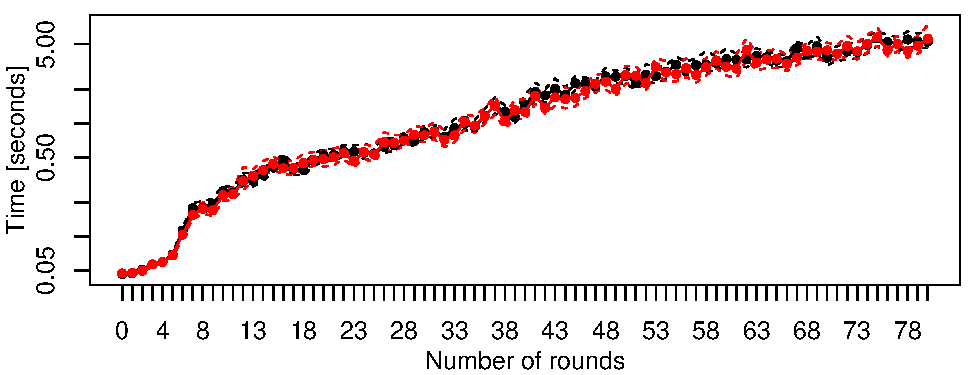
\includegraphics[width=.5\textwidth]{figures/opt-sha1/sha1-32bit-8bitref-cmp-espresso.pdf}
\caption{Mean running time and 95\% confidence intervals for $8$-bit preimage attack on \emph{SHA-1} without optimizations (black) and using \emph{Espresso} minimization for rounds functions (red).}
\label{fig:opt-sha1-cmp-espresso}
\end{figure}
 
Figure \ref{fig:opt-sha1-cmp-espresso} shows the mean running times for both instances without optimizations and for ones using \emph{Espresso} minimization.
As we can see the effect of this optimization is quite small and the running times appear to be identical.

%TODO nejaka tabulka a cisla?
%TODO mozno porovnat aj pocet konfliktov/velkost instancie s a bez opt?

Using the \emph{Games-Howell} post hoc test we do obtain a mean time improvement of $t=1.4$ seconds however at a fairly high significance level of $p=0.15$ which does not give us enough evidence to reject the hypothesis that this optimization leads to no improvement.

TODO pre viac ako x kol iba?
%TODO reference G-H

\subsubsection{SHA-3 analysis} 
We performed a similar experiment for the \emph{SHA-3} hash function, finding an $8$-bit preimage on $32$-bit message where the preimage bits again came from randomly generated messages.
We considered two possible optimizations in the round function and tested four variants -- all combinations of turning on or off these two optimizations.
A total of $2000$ samples was collected for each variant.

The first optimization was minimizing the expression $x \oplus (\overline{y} \land z)$ in the $\chi$ step, which is used to fill the $5\times 5$ state matrix $S$ in each round.

The second optimization was in the $\theta$ step, where the $C$ vector is filled using an exclusive or of five different values.
Without optimization this leads to four extra variables and 16 extra clauses.
Using the \emph{Espresso} minimization will lead to 32 clauses but only one extra variable.

Using the \emph{Games-Howell} procedure again we obtain the pairwise comparison shown in table \ref{tbl:opt-sha3-cmp}.

TODO pekna tabulka
TODO tiezlen pre >12 kol?

We can see that the \emph{xor} optimization -- which reduces the number of variables but requires twice as many clauses -- in fact leads to higher solving time (mean difference $t=3.1$) at significance level of $p=0.01$.
Thus the default behavior is more efficient.
On the other hand, from the high p-value of $0.96$ we can't reject the hypothesis that optimizing the $\chi$ step makes no difference at all.

%\begin{figure}
%\begin{tabular}{c|c|c|c|c}
%
%\end{tabular}
%\label{tbl:opt-sha3-cmp}
%\end{figure}

\subsubsection{Discussion}
Even with large number of samples to eliminate the intrinsic randomness in SAT solving times we were unable to reject hypotheses that the tested optimizations do not lead to an improvement.
From this we conclude that they do not provide significant benefits.

While our library provides this optimization feature to users as we saw in our measurements it is not necessary to use it.
Therefore minimal changes to existing, off-the-shelf implementations of hash functions (without the need to identify expressions with non-optimal Tseitin representation) are sufficient to match the hand-optimized instances such as in \cite{nossum2012sat}.
%TODO discussion/conclusion
%TODO high pvalue, no difference -> parada, netreba to pouzivat, nasa naive noeffort kniznica je rovnako dobra ako handcrafted kod

%\subsection{Merging operators}
%TODO ~0.25pgs

%\subsection{Truth table minimization}
%TODO ~1pgs + nejake porovnania velkosti a rychlosti

\subsection{Branching order}
\label{sec:branching-order}
%TODO nossum/soos mailing list cite; is it in text?; more references to literature

The most important heuristic in a SAT solver is the decision which unassigned variable to pick next.
A bad order might assign randomly picked values to many variables before some conflict is found and the search tree depth will be quite high.
This in turn leads to an increased solving time.
On the other hand a good heuristic would pick variables in an order that causes many propagations and with an unsatisfiable assignment leads to conflicts quickly.

The branching order is picked by a heuristic in the SAT solver, which does not have additional knowledge about what these variables represent and how they relate to each other.
By extending the input file format and the variable picking algorithm we can provide our own (partial) variable branching order.

\subsubsection{Implementation}
\label{sec:branching-order-impl}
We added a new input line type to the \emph{DIMACS CNF} file format.
A line in the form

\centerline{\texttt{b $v$ 0}}

\noindent means that variable $v$ should be branched on first.
When multiple such lines are provided the order of branching is the same as the order of these lines in the input file.
Using this we can provide a list of any number of variables in the order we want them to be picked for assignment.

We modified the popular \emph{MiniSat} solver to be able to parse and store this list.
Then we modified the selection of next branching candidate to first pick all these variables in the specified order.
Once all have been assigned we fall back to the standard branching order algorithm.

We have also added support for this to our modeling library.
Before the boolean circuit is transformed to a set of CNF clauses and written to a file, the user can specify arbitrary branching order using variables defined in the model of the cryptographic primitive.

\subsubsection{SHA-3 analysis}
For \emph{SHA-3-512} we tested various branching orders on $8$-bit reference preimage attack with number of rounds ranging from $0$ to $24$ (full SHA-3).
For every number of rounds 10 different instances were generated and each was solved 10 times, for a total of 100 samples per round per strategy.
We compared the following branching order strategies:

\textbf{\emph{none}}: No branching order was specified. This is the default unmodified \emph{MiniSat} behavior.

\textbf{\emph{r0-S-x-y}}: The $S$ matrix from the first round is branched on first, in column-major order.

\textbf{\emph{r0-S-y-x}}: Same as previous one, but in row-major order.

\textbf{\emph{rlast-S-x-y}} and \textbf{\emph{rlast-S-y-x-}}: Same as previous two, but the $S$ matrix from the last round is used instead.	

\begin{figure}
\centering 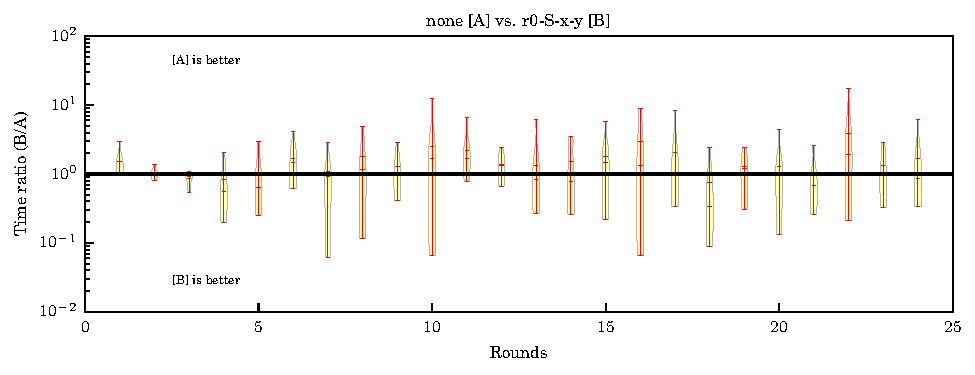
\includegraphics{figures/bo-ex1/ratio-time-none-r0sxy.pdf}
\caption{Violin plot showing the distribution of time ratios.}
\label{fig:bo-ratio-time-none-r0sxy}
\end{figure}

\begin{figure}
\centering 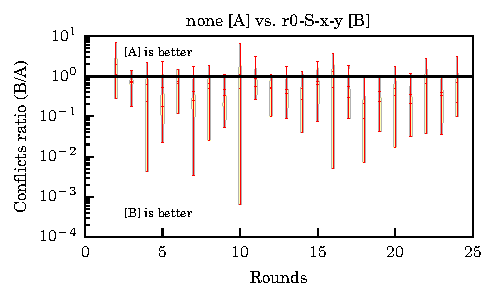
\includegraphics{figures/bo-ex1/ratio-confl-none-r0sxy.pdf}
\caption{Violin plot showing the distribution of number of conflict ratios.}
\label{fig:bo-ratio-confl-none-r0sxy}
\end{figure}

The figures \ref{fig:bo-ratio-time-none-r0sxy} and \ref{fig:bo-ratio-confl-none-r0sxy} show \emph{violin plots} of the distribution of ratios of the solving time and the number of conflicts.
Each \emph{violin} also show the mean, median and extreme values.

From these plots we see that while the ratios for the number of conflict are mostly below 1 (meaning that the \emph{r0-S-x-y} strategy leads to fewer conflicts), the time ratios are often higher than 1.

The \emph{Games-Howell} procedure confirms these findings, with the mean difference for number of conflicts between the \emph{none} and \emph{r0-S-x-y} strategies of $t = 21$ at significance level $p < 0.001$.
However, for the solving time the high p-value does not let us reject the hypothesis that any difference is due to chance.

TODO GH tabulka cas/konflikty pre rounds>12 (odstrani sum)
TODO spomenut ze len pre rounds>12

The \emph{r0-S-y-x} strategy behaves the same as \emph{r0-S-x-y} -- the number of conflicts for every instance is identical and the differences in time are negligible.

TODO preco?

On the other hand the strategies starting with the last round's $S$ matrix lead to the same behavior as not providing any branch ordering at all (the \emph{none} strategy).
This must mean that either their choice does not lead to any forced assignments and conflicts (which is highly unlikely) or that the default \emph{MiniSat} heuristic is also picking them for branching first.

TODO aj ine verzie ako r0-C, D, ... ziaden efekt/rovnake ako S


\subsubsection{Discussion}

TODO prepisat koniec predoslej casti a dat to sem, + najaky kratky sumar	
%A possible branch ordering would be based on the rounds of a hash function.
%Given the reduced 20 rounds variant of SHA-1, we could first force the solver to assign values to all variables corresponding to variables in the $n$-th round of the compression function.
%
%By trying various orders we obtain the results shown in Figure \ref{fig:opt-branchorder-example-sha1}-branchorder-example-sha1}.
%The numbers in the \emph{order} column refer to the rounds of the compression function.
%For example \emph{20, 19} means that first all variables from the 20th round get assigned, then all variables from 19th round and then the original heuristic takes over.
%
%While the times are averages over multiple runs they are still quite small and susceptible to random noise.
%However the number of conflicts is a more reliable measure and we can see interesting trends from this small example.
%Forcing the SAT solver to work backwards (20, 19, 18) is much worse than the general heuristic.
%On the other hand, starting with the first round leads to significant speed-up.
%
%\begin{figure}
%\caption{Solving time and number of conflicts for 8-bit preimage with 32-bit message on reduced 20-rounds SHA-1 with various branching orders.}
%\label{fig:opt-branchorder-example-sha1}
%\begin{tabular}{l|c|c}
%Order & Time [s] & Conflicts \\ \hline
%--- & 0.96 & 9755 \\ \hline
%20 & 0.94 & 9755 \\
%20, 19 & 0.97 & 9755 \\
%20, 19, 18 & 17.35 & 71197 \\ \hline
%1 & 0.35 & 1062 \\
%2 & 0.35 & 1062 \\
%1, 2 & 0.33 & 1062 \\
%1, 2, 3 & 0.29 & 927 \\
%1, 2, 3, 4 & 0.28 & 185 \\
%1, 4 & 0.24 & 119
%\end{tabular}
%\end{figure}
%TODO nicer table, new numbers with averages
%TODO rerun these numbers with more rounds? with more trials for better averages? and (!!!) with equal seed distributions (generate ~1k seeds, run each order with the same ones)
%TODO proper systematic evaluation
%TODO implement groups for branch ordering? might be slower due to complex selection...
\chapter{Experiments}

In this chapter we describe various experiments that were performed to evaluate the effectiveness and necessity of optimizations described in the previous chapter.
These experiments compare the time required to solve particular instances across two or more variants.
Each variant can either a modification to the instance itself (by changing the way it is generated) or the instance can be unchanged but rather the behavior of the SAT solver itself is modified.

\section{Methodology}
Since the running time of a SAT solver is not deterministic it is not enough to simply perform a single run for every instance.
In fact, given the same instance and same SAT solver the running time can differ significantly, even by several orders of magnitude.
We will therefore need to gather multiple samples and use sound statistical methods to discover patterns in this noisy data.

\subsubsection{Sampling procedure}
To counter the high variability in time even for one instance we will solve each instance several times.

Additionally, not all instances for particular parameters (such as number of rounds) are equally hard.
For example, reduced hash functions with number of rounds significantly lower than the full hash function do not behave sufficiently as random functions.
Some output digests might be significantly less likely to be produced than other, or might not be even be possible.
When we are performing a partial preimage attack by fixing several digest bits to be equal to a reference digest (obtained by first hashing a random message) some instances might have fewer solutions than others and be therefore harder.

For this reason we will also perform all such experiments on multiple instances, that have identical parameters but the random reference messages are independently generated.

\subsubsection{Censoring}
Sometimes we might obtain an instance that takes very long time to solve.
To ensure that experiments conclude in a reasonable time it is common to enforce a time limit and abort all computations that exceed it.
Since in such cases we can not know the true running time we must discard these aborted measurements.

Data sets with such discarded measurements are called \emh{censored}.
They make statistical analysis complicated if not impossible, since even trivial statistics such as mean can not be computed without knowing the true censored values.

For this reason we avoided censoring in our experiments.
While we did have a time limit in place, all experiments that contained censored runs were discarded and not considered for analysis.
To obtain valid experiments we either increased the time limit or reduced some of the parameters (such as number of rounds or length of the preimage) until we got a configuration that finished without any censoring.

\subsubsection{Statistical analysis}



\section{Expression encoding evaluation}
...
\subsection{SHA-1 analysis}
We evaluated the effectiveness of this optimization on preimage attacks on \emph{SHA-1} using the unmodified Tseitin encoding and using the \emph{Espresso} optimizer on both the \emph{choice} and \emph{majority} round functions.
We measured the running time of finding an $8$-bit preimage for $32$-bit input message.
The preimage bits were obtained by hashing random messages to ensure a solution would exist even for instances with reduced number of rounds.
We repeated the experiment multiple times for a total of $5670$ samples for each variant.
 
Figure \ref{fig:opt-sha1-cmp-espresso} shows the mean running times for both instances without optimizations and for ones using \emph{Espresso} minimization.
As we can see the effect of this optimization is quite small and the running times appear to be identical.

%> posthocTGH(y=raw[raw$rounds>20,]$time, x=raw[raw$rounds>20,]$label, method='games-howell')
%          n means variances
%s1espr 4200   2.5       7.4
%s1none 4200   2.6       7.4
%
%                t   df    p
%s1espr:s1none 1.6 8398 0.12

Using the \emph{Games-Howell} post hoc test \cite{games1976pairwise} on instances with more than $20$ rounds (to reduce the effect of randomness when measuring very short time intervals) we do obtain a mean time improvement of $t=1.6$ seconds however at a fairly high significance level of $p=0.12$ which does not give us enough evidence to reject the hypothesis that this optimization leads to no improvement.

\subsection{SHA-3 analysis} 
\label{sec:sha3-espresso}

%> posthocTGH(y=raw[raw$rounds>12,]$time, x=raw[raw$rounds>12,]$label, method='games-howell')
%          n means variances
%s3esno  949   7.4        50
%s3esxor 949   8.2        54
%s3nono  949   7.5        45
%s3noxor 949   8.5        49
%
%                   t   df      p
%s3esno:s3esxor  2.56 1892 0.0521
%s3esno:s3nono   0.52 1891 0.9540
%s3esno:s3noxor  3.63 1896 0.0016
%s3esxor:s3nono  2.11 1878 0.1499
%s3esxor:s3noxor 0.98 1891 0.7581
%s3nono:s3noxor  3.21 1892 0.0075
\begin{figure*}
\centering \begin{tabular}{ccrccrr}
\multicolumn{2}{c}{\textbf{Optimizations}} & \multicolumn{1}{c}{\textbf{Time}} & \multicolumn{2}{c}{\textbf{Optimizations}} & \multicolumn{2}{c}{\textbf{Time}} \\
\textbf{$\chi$ step} & \textbf{$\theta$ step} & \multicolumn{1}{c}{\textbf{Mean}} & \textbf{$\chi$ step} & \textbf{$\theta$ step} & \textbf{t} & \textbf{p}\\ \hline
\xmark & \xmark & $7.5$ & \xmark & \cmark & $3.21$ & $<0.01$ \\
& & & \cmark & \xmark & $0.52$ & $0.95$ \\
& & & \cmark & \cmark & $2.11$ & $0.15$ \\ \hline
\xmark & \cmark & $8.5$ & \cmark & \xmark & $3.63$ & $<0.01$ \\
& & & \cmark & \cmark & $0.98$ & $0.75$ \\ \hline
\cmark & \xmark & $7.4$ & \cmark & \cmark & $2.56$ & $0.05$ \\ \hline
\cmark & \cmark & $8.2$ & \\
\end{tabular}
\caption{Pairwise comparison of four \emph{SHA-3-512} optimization combinations using the Games-Howell procedure. Only measurements for more than $12$ rounds were used to avoid randomness in timing, for a total of $n=949$ samples per strategy.}
\label{tbl:gh-sha3-opts}
\end{figure*}

We performed a similar experiment for the \emph{SHA-3} hash function, finding an $8$-bit preimage on $32$-bit message where the preimage bits again came from randomly generated messages.
We considered two possible optimizations in the round function and tested four variants -- all combinations of turning on or off these two optimizations.
A total of $2000$ samples was collected for each variant.

The first optimization was minimizing the expression $x \oplus (\overline{y} \land z)$ in the $\chi$ step, which is used to fill the $5\times 5$ state matrix $S$ in each round.

The second optimization was in the $\theta$ step, where the $C$ vector is filled using an exclusive or of five different values.
Without optimization this leads to four extra variables and 16 extra clauses.
Using the Espresso minimization will lead to 32 clauses but only one extra variable.

Using the Games-Howell procedure again we obtain the pairwise comparison shown in figure \ref{tbl:gh-sha3-opts}.

We can see that the \emph{xor} optimization -- which reduces the number of variables but requires twice as many clauses -- in fact leads to higher solving time (mean difference $t=3.21$) at significance level of $p < 0.01$.
Thus the default behavior is more efficient.
On the other hand, from the high p-value of $0.75$ we can't reject the hypothesis that optimizing the $\chi$ step makes no difference at all.

\subsection{Discussion}
Even with large number of samples to eliminate the intrinsic randomness in SAT solving times we were unable to reject hypotheses that the tested optimizations do not lead to an improvement.
From this we conclude that they do not provide significant benefits.

While our library provides this optimization feature to users as we saw in our measurements it is not necessary to use it.
Therefore minimal changes to existing, off-the-shelf implementations of hash functions (without the need to identify expressions with non-optimal Tseitin representation) are sufficient to match the hand-optimized instances such as in \cite{nossum2012sat}.

\begin{figure*}	
\centering 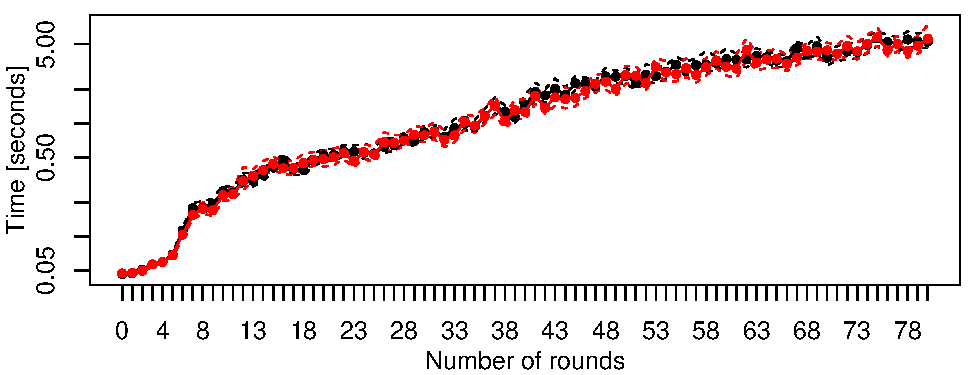
\includegraphics{figures/opt-sha1/sha1-32bit-8bitref-cmp-espresso.pdf}
\caption{Mean running time and 95\% confidence intervals for $8$-bit preimage attack on \emph{SHA-1} without optimizations (black) and using Espresso minimization for rounds functions (red).}
\label{fig:opt-sha1-cmp-espresso}
\end{figure*}

\begin{figure*}
\centering 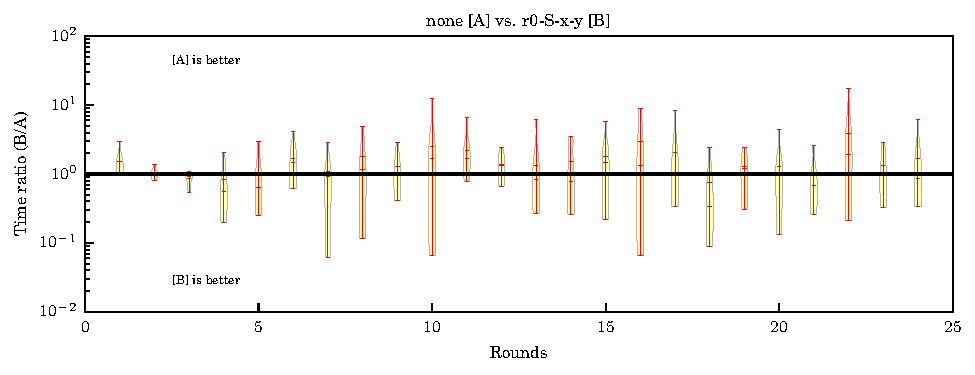
\includegraphics{figures/bo-ex1/ratio-time-none-r0sxy.pdf}
\caption{Violin plot showing the ratios distribution of solving time for the \emph{none} and \emph{r0-S-x-y} strategies.}
\label{fig:bo-ratio-time-none-r0sxy}
\end{figure*}

\begin{figure*}
\centering 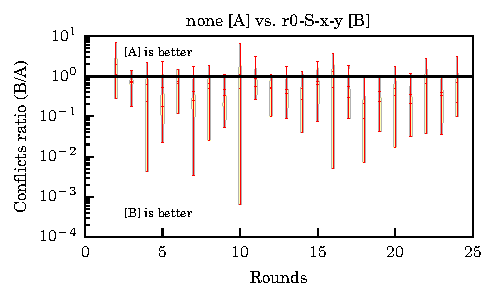
\includegraphics{figures/bo-ex1/ratio-confl-none-r0sxy.pdf}
\caption{Violin plot showing the ratios distribution of number of conflicts for the \emph{none} and \emph{r0-S-x-y} strategies.}
\label{fig:bo-ratio-confl-none-r0sxy}
\end{figure*}

\section{Branching order evaluation}
...
\subsection{SHA-3 analysis}
For \emph{SHA-3-512} we tested various branching orders on $8$-bit reference preimage attack with number of rounds ranging from $0$ to $24$ (full SHA-3).
For every number of rounds 10 different instances were generated and each was solved 10 times, for a total of 100 samples per round per strategy.
We compared the following branching order strategies:

\textbf{\emph{none}}: No branching order was specified. This is the default unmodified MiniSat behavior.

\textbf{\emph{r0-S-x-y}}: The $S$ matrix from the first round is branched on first, in column-major order.

\textbf{\emph{r0-S-y-x}}: Same as previous one, but in row-major order.

\textbf{\emph{rlast-S-x-y}} and \textbf{\emph{rlast-S-y-x-}}: Same as previous two, but the $S$ matrix from the last round is used instead.	

The figures \ref{fig:bo-ratio-time-none-r0sxy} and \ref{fig:bo-ratio-confl-none-r0sxy} show \emph{violin plots} of the distribution of ratios of the solving time and the number of conflicts.
Each \emph{violin} also show the mean, median and extreme values.

From these plots we see that while the ratios for the number of conflict are mostly below 1 (meaning that the \emph{r0-S-x-y} strategy leads to fewer conflicts), the time ratios are often higher than 1.

%> posthocTGH(y=confl[confl$rounds>12,]$time, x=confl[confl$rounds>12,]$label, method='games-howell')
%              n means variances
%none        480   731    330234
%r0-S-x-y    480   250     51256
%r0-S-y-x    480   250     51256
%rlast-S-x-y 480   731    330234
%rlast-S-y-x 480   731    330234
%
%                         t  df       p
%none:r0-S-x-y           17 624 1.7e-10
%none:r0-S-y-x           17 624 1.7e-10
%none:rlast-S-x-y         0 958 1.0e+00
%none:rlast-S-y-x         0 958 1.0e+00
%r0-S-x-y:r0-S-y-x        0 958 1.0e+00
%r0-S-x-y:rlast-S-x-y    17 624 1.7e-10
%r0-S-x-y:rlast-S-y-x    17 624 1.7e-10
%r0-S-y-x:rlast-S-x-y    17 624 1.7e-10
%r0-S-y-x:rlast-S-y-x    17 624 1.7e-10
%rlast-S-x-y:rlast-S-y-x  0 958 1.0e+00
%> posthocTGH(y=time[time$rounds>12,]$time, x=time[time$rounds>12,]$label, method='games-howell')
%              n means variances
%none        480   7.8        35
%r0-S-x-y    480   7.5        39
%r0-S-y-x    480   7.5        38
%rlast-S-x-y 480   7.8        36
%rlast-S-y-x 480   7.8        35
%
%                            t  df    p
%none:r0-S-x-y           0.647 956 0.97
%none:r0-S-y-x           0.576 956 0.98
%none:rlast-S-x-y        0.185 958 1.00
%none:rlast-S-y-x        0.032 958 1.00
%r0-S-x-y:r0-S-y-x       0.071 958 1.00
%r0-S-x-y:rlast-S-x-y    0.826 956 0.92
%r0-S-x-y:rlast-S-y-x    0.680 956 0.96
%r0-S-y-x:rlast-S-x-y    0.755 957 0.94
%r0-S-y-x:rlast-S-y-x    0.609 956 0.97
%rlast-S-x-y:rlast-S-y-x 0.153 958 1.00
\begin{figure*}
\centering \begin{tabular}{lrrlrrrr}
\textbf{Strategy} & \textbf{Time} & \textbf{Conflicts} & \textbf{Strategy} & \multicolumn{2}{c}{\textbf{Time}} & \multicolumn{2}{c}{\textbf{Conflicts}} \\
& \multicolumn{2}{c}{\textbf{Mean}} & & \textbf{t} & \textbf{p} & \textbf{t} & \textbf{p} \\ \hline
\emph{none} & $7.8$ & $731$ & \emph{r0-S-x-y} & $0.65$ & $0.97$ & $17$ & $<0.01$ \\
& & & \emph{r0-S-y-x} & $0.58$ & $0.98$ & $17$ & $<0.01$ \\
& & & \emph{rlast-S-x-y} & $0.18$ & $>0.99$ & $958$ & $>0.99$ \\
& & & \emph{rlast-S-y-x} & $0.03$ & $>0.99$ & $958$ & $>0.99$ \\ \hline
\emph{r0-S-x-y} & $7.5$ & $250$ & \emph{r0-S-y-x} & $0.07$ & $>0.99$ & $0$ & $<0.01$ \\	
& & & \emph{rlast-S-x-y} & $0.83$ & $0.92$ & $17$ & $<0.01$ \\
& & & \emph{rlast-S-y-x} & $0.68$ & $0.96$ & $17$ & $<0.01$ \\ \hline
\emph{r0-S-y-x} & $7.5$ & $250$ & \emph{rlast-S-x-y} & $0.76$ & $0.94$ & $17$ & $<0.01$ \\
& & & \emph{rlast-y-x} & $0.60$ & $0.97$ & $17$ & $<0.01$ \\ \hline
\emph{r0-last-x-y} & $7.8$ & $731$ & \emph{rlast-S-y-x} & $0.15$ & $>0.99$ & $0$ & $>0.99$ \\ \hline
\emph{r0-last-y-x} & $7.8$ & $731$ & & & & &  \\
\end{tabular}
\caption{Pairwise comparison of various branching order strategies for \emph{SHA-3-512} using the Games-Howell procedure. Only measurements for more than $12$ rounds were used to avoid randomness in timing for a total of $n=480$ samples per strategy.}
\label{tbl:gh-sha3-bos}
\end{figure*}

The Games-Howell procedure (figure \ref{tbl:gh-sha3-bos}) confirms these findings, with the mean difference for number of conflicts between the \emph{none} and \emph{r0-S-x-y} strategies of $t = 17$ at significance level $p < 0.01$.
However, for the solving time the high p-value does not let us reject the hypothesis that any difference is due to chance.
Note that once again only samples for more than $12$ rounds were included to avoid the strong effect of randomness for instances that solve in very short time.

The \emph{r0-S-y-x} strategy behaves the same as \emph{r0-S-x-y} -- the number of conflicts for every instance is identical and the differences in time are negligible.
On the other hand the strategies starting with the last round's $S$ matrix lead to the same behavior as not providing any branch ordering at all (the \emph{none} strategy).

Similar experiments were performed with the auxiliary vectors and matrices $B, C$ and $D$ with the same results -- enforcing branching order did not lead to better solving times.

\subsection{Discussion}

The fact that these branching order do not change the solving time significantly must mean that either their choice does not lead to any forced assignments and conflicts (which is highly unlikely) or that the default MiniSat heuristic is also picking them for branching first.
The second case means that this optimization is unnecessary and that the default SAT solver heuristic is sufficient in this case.
%\unnumberedchapter{Conclusion}
\chapter{Conclusions}
We have created a library for modeling various problems as SAT instances that can then be solved with SAT solvers.
While the library is fairly universal we have specifically focused on cryptographic problems such as modeling preimage attacks on hash functions.
To simplify this use case we make use of operator overloading that allows using our library with existing implementations with minimal changes.

Previous works in this area used handwritten code to generate instances of a specific hash function that were not easily modifiable.
However this allowed them to optimize the resulting instances, reducing the number of variables and clauses required compared to a na\"{\i}ve Tseitin transformation.
We added an option to optimize specific expression to our library and evaluated the effects of those optimizations.

While we found that the optimized instances can lead to fewer conflicts the solving time was not improved in any statistically significant way.
This leads us to conclude that these optimizations are not required and therefore the minimal changes to existing implementations mentioned above are sufficient to create a reasonable instance.

We then modified the MiniSat solver to see if overriding the default branching order heuristic with the help of additional information about the problem structure would lead to speed improvements.
However, same as with previous optimizations, we found that only the number of conflicts was reduced in this way.
From this we conclude that the existing heuristics employed by modern solvers behave reasonably on these instances and therefore using an off-the-shelf solver is sufficient.
%
%
%\unnumberedchapter{Introduction}
%
%\chapter{Background}

%\chapter{Related Work}
%
%\chapter{Approach Overview}
%\chapter{Library design}
%\chapter{Library use}
%
%\chapter{Heuristics}
%\chapter{Measurements}
%\chapter{Analysis}
%
%%\unnumberedchapter{Conclusion}
\chapter{Conclusions}
We have created a library for modeling various problems as SAT instances that can then be solved with SAT solvers.
While the library is fairly universal we have specifically focused on cryptographic problems such as modeling preimage attacks on hash functions.
To simplify this use case we make use of operator overloading that allows using our library with existing implementations with minimal changes.

Previous works in this area used handwritten code to generate instances of a specific hash function that were not easily modifiable.
However this allowed them to optimize the resulting instances, reducing the number of variables and clauses required compared to a na\"{\i}ve Tseitin transformation.
We added an option to optimize specific expression to our library and evaluated the effects of those optimizations.

While we found that the optimized instances can lead to fewer conflicts the solving time was not improved in any statistically significant way.
This leads us to conclude that these optimizations are not required and therefore the minimal changes to existing implementations mentioned above are sufficient to create a reasonable instance.

We then modified the MiniSat solver to see if overriding the default branching order heuristic with the help of additional information about the problem structure would lead to speed improvements.
However, same as with previous optimizations, we found that only the number of conflicts was reduced in this way.
From this we conclude that the existing heuristics employed by modern solvers behave reasonably on these instances and therefore using an off-the-shelf solver is sufficient.


\backmatter
    \printbibliography
    
    %\clearpage
\pagestyle{empty}
\null\vfil

\begin{adjustwidth}{2cm}{2cm}
\begin{center}
{\LARGE\textsf{Colophon}}

\noindent This thesis was typeset using \textsf{\XeLaTeX} with the \textsf{memoir} package for layout, \textsf{\textsc{minted}} for code samples and \textsf{\textsc{Bib}\LaTeX} with \textsf{\textsc{biber}} for bibliography. Figures were created using \textsf{Ti\textit{k}Z/PGF}, \textsf{\textsc{matplotlib}} and \textsf{\textsc{R}}.

\vspace{2cm}

%\begin{center}
{\Large \ccbysa}
%\end{center}

\noindent Text of this thesis is released under the \textsf{Creative Commons BY-SA 4.0} license, the full text of which can be found at\\
\url{https://creativecommons.org/licenses/by-sa/4.0/}.

\vspace{1cm}

\noindent Source code for this text including all illustrations is available at \url{https://github.com/lacop/master-thesis-text}.
\end{center}
\end{adjustwidth}

\vfil
\end{document}